\section{Object detection and segmentation}
\label{sec:ch2_detection}

This thesis targets real-time robotic brick picking, which requires both accurate localization and reliable instance boundaries. Object detection provides coarse localization via bounding boxes, while instance segmentation adds pixel-level masks that improve geometric reasoning, overlap handling, and downstream grasp selection. One-stage detectors in the YOLO family are popular in such settings because they perform dense predictions in a single forward pass, enabling high throughput with competitive accuracy. The reference study evaluates YOLOv8 for instance segmentation and emphasizes its practicality for real-world imagery, including challenging scenes with occlusion and clutter. \cite{sapkota2024yolov8v11}

\subsection{YOLOv8 Instance Segmentation Overview}
YOLOv8 extends a detection pipeline with a segmentation branch that predicts per-instance masks in addition to bounding boxes. The model follows a backbone--neck--head structure:
\begin{itemize}
    \item \textbf{Backbone}: extracts multi-scale features from the input image using stacked convolutional blocks and residual-style pathways to preserve gradient flow and capture context across receptive fields.
    \item \textbf{Neck}: aggregates features across multiple resolutions to improve sensitivity to objects of different sizes, which is critical when bricks appear at varying scales in the workspace.
    \item \textbf{Head}: predicts class scores and bounding box regression from fused features using an anchor-free design, reducing dependence on hand-crafted anchor configurations. \cite{sapkota2024yolov8v11}
\end{itemize}
The segmentation branch runs in parallel to the detection head and produces instance masks, enabling pixel-level delineation of brick contours. This design is suitable for robotic perception because it balances segmentation accuracy with real-time requirements. \cite{sapkota2024yolov8v11}

\subsection{Segmentation Head and Mask Generation}
YOLOv8 segmentation models generate object masks by combining learned mask representations with instance-specific coefficients. Conceptually, the segmentation head predicts a set of mask prototypes at a reduced resolution, and each detected instance is assigned coefficients that linearly combine these prototypes into a final mask. This approach is computationally efficient because the expensive mask computation is shared across instances, while instance-specific coefficients remain lightweight. The reference study highlights YOLOv8 as a strong accuracy--speed trade-off for instance segmentation in practical imaging conditions. \cite{sapkota2024yolov8v11}

\subsection{Inference Pipeline and Real-Time Considerations}
During inference, YOLOv8 produces dense predictions across spatial locations and then filters detections based on confidence scores, followed by non-maximum suppression to remove redundant boxes. The segmentation outputs are aligned with the selected detections to generate final instance masks. This end-to-end pipeline is efficient and supports real-time operation, which is critical for the closed-loop perception and control in robotic manipulation. \cite{sapkota2024yolov8v11}

\subsection{Model Choice for This Thesis (YOLOv8s-seg)}
Based on the reference evaluation of YOLOv8 for instance segmentation, this thesis adopts \textbf{YOLOv8s-seg}, the small segmentation variant. The \emph{s} model size provides a favorable balance between speed and accuracy, making it suitable for on-line inference with limited computational resources. The segmentation capability is particularly valuable for bricks because it provides accurate outlines that help refine grasp candidate selection and reduce ambiguity when bricks are partially occluded or closely packed. \cite{sapkota2024yolov8v11}

\begin{figure}[H]
    \centering
    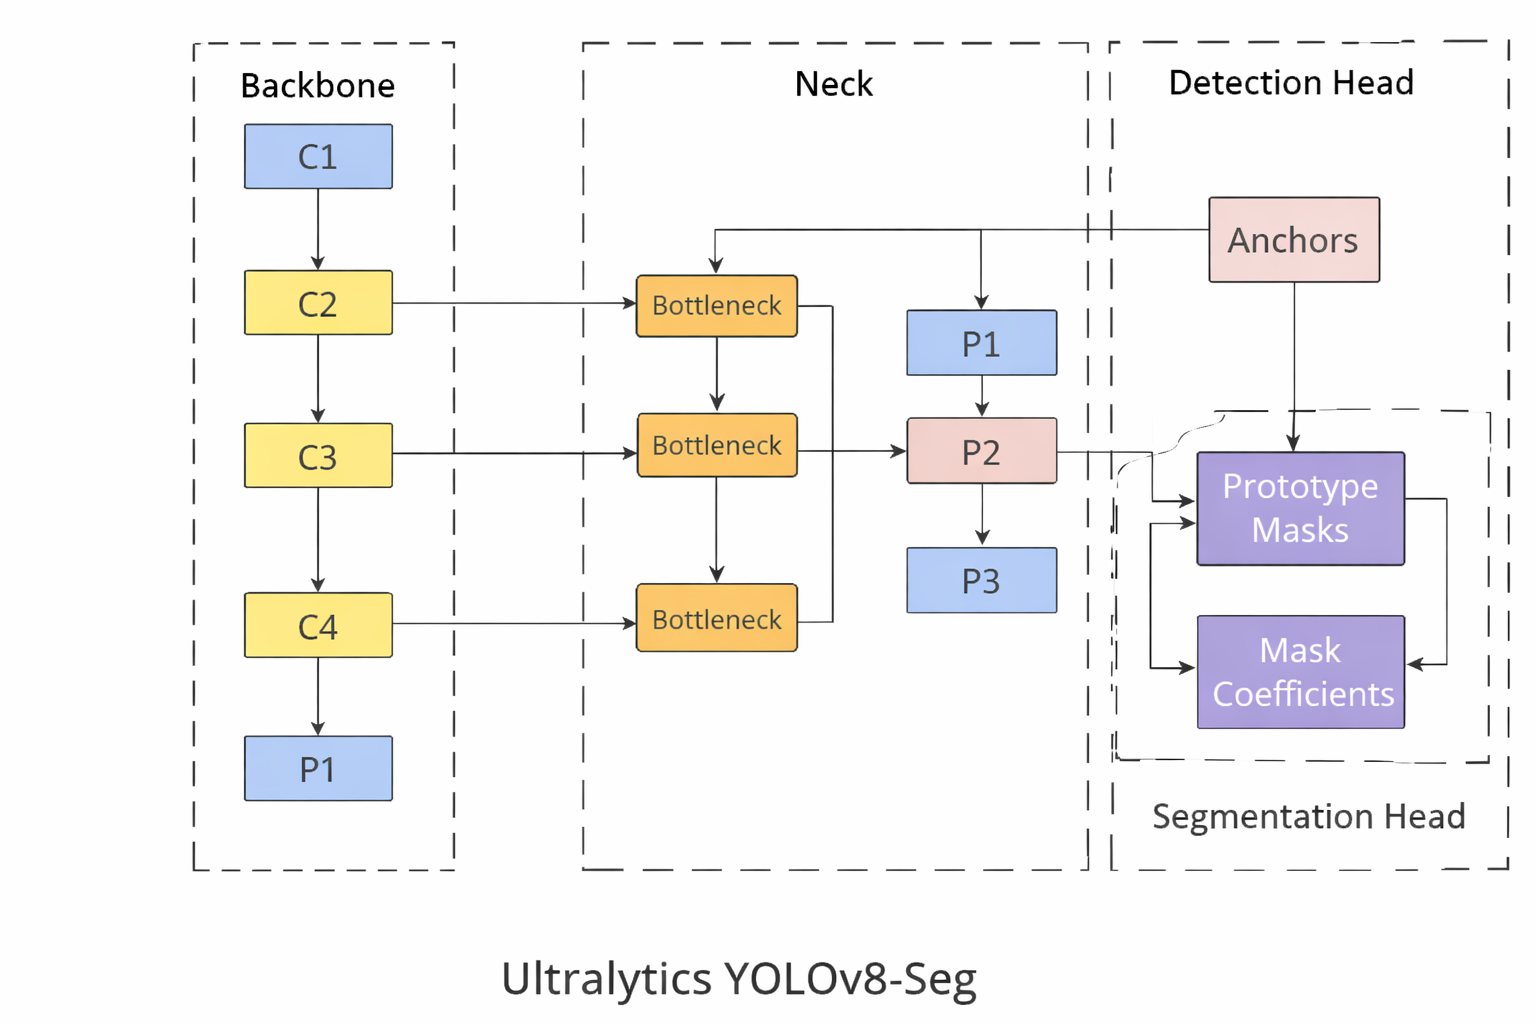
\includegraphics[width=0.9\textwidth]{Figures/chapter2/Detection/yolov8s_seg_arch.png}
    \caption{YOLOv8s-seg architecture overview (based on Ultralytics YOLOv8-seg documentation). \cite{ultralytics_yolov8_docs}}
    \label{fig:yolov8s_seg_arch}
\end{figure}
